% 外角定理：外角等于两不相邻内角之和
\documentclass[tikz,border=4pt]{standalone}
\usepackage{ctex}
\usepackage{amsmath}
\usetikzlibrary{calc}
\begin{document}
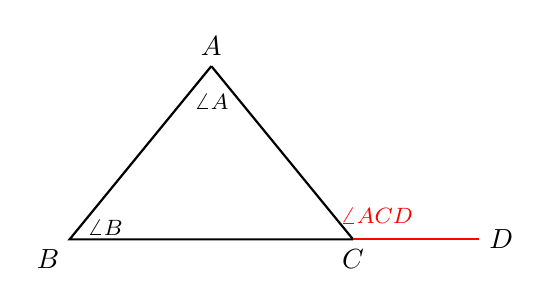
\begin{tikzpicture}[scale=1.0, thick]
  \coordinate (A) at (0, 2.2);
  \coordinate (B) at (-1.8, 0);
  \coordinate (C) at (1.8, 0);
  \coordinate (D) at (3.4, 0);  % 延长 BC 到 D
  \draw (A) -- (B) -- (C);
  \draw (A) -- (C);
  \draw[red] (C) -- (D);

  \node[above] at (A) {$A$};
  \node[below left] at (B) {$B$};
  \node[below] at (C) {$C$};
  \node[right] at (D) {$D$};

  \node at ($(B)+(0.45, 0.15)$) {\footnotesize $\angle B$};
  \node at ($(A)+(0,   -0.45)$) {\footnotesize $\angle A$};
  \node[red] at ($(C)+(0.3, 0.3)$) {\footnotesize $\angle ACD$};
\end{tikzpicture}
\end{document}
